\documentclass[tikz,border=2pt]{standalone}
\usepackage{amsmath}
\usepackage{pgfplots}
\pgfplotsset{compat=1.18}
\usetikzlibrary{arrows.meta,calc}
\begin{document}
% Theorem 5.1 on Example 5.1: (P) -> dual (D) -> (D) in standard form -> its dual, which after changing all signs is (P) again.
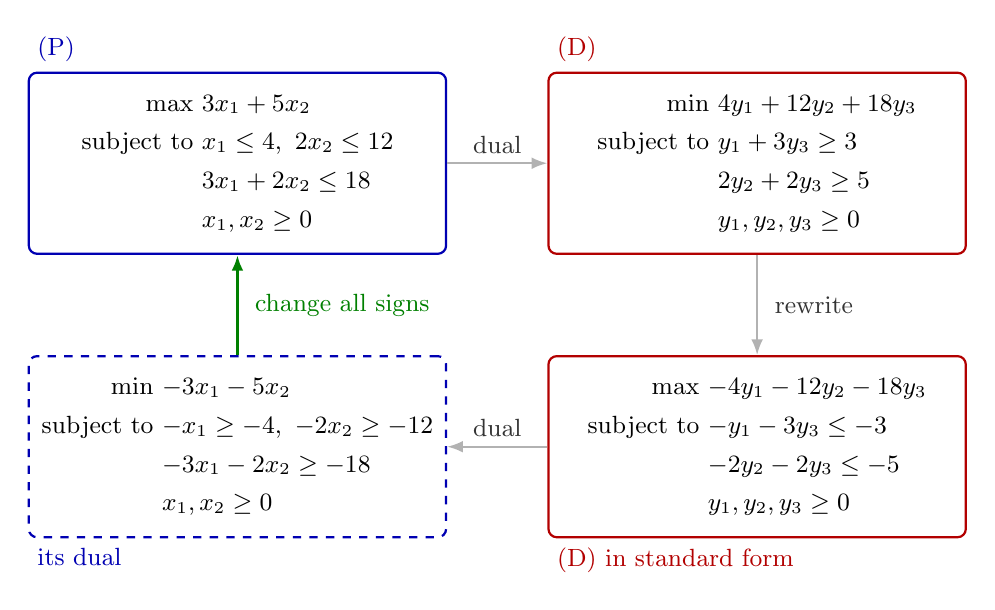
\begin{tikzpicture}[font=\small, >={Latex[length=2mm]},
    lp/.style={draw, rounded corners=3pt, thick, minimum width=5.3cm, minimum height=2.3cm, align=left}]
  \node[lp, blue!70!black, text=black] (P) at (0,0) {$\begin{aligned}\max\ & 3x_1+5x_2\\ \text{subject to}\ & x_1\leq4,\ 2x_2\leq12\\ & 3x_1+2x_2\leq18\\ & x_1,x_2\geq0\end{aligned}$};
  \node[lp, red!70!black, text=black] (D) at (6.6,0) {$\begin{aligned}\min\ & 4y_1+12y_2+18y_3\\ \text{subject to}\ & y_1+3y_3\geq3\\ & 2y_2+2y_3\geq5\\ & y_1,y_2,y_3\geq0\end{aligned}$};
  \node[lp, red!70!black, text=black] (Ds) at (6.6,-3.6) {$\begin{aligned}\max\ & {-}4y_1-12y_2-18y_3\\ \text{subject to}\ & {-}y_1-3y_3\leq-3\\ & {-}2y_2-2y_3\leq-5\\ & y_1,y_2,y_3\geq0\end{aligned}$};
  \node[lp, blue!70!black, dashed, text=black] (DD) at (0,-3.6) {$\begin{aligned}\min\ & {-}3x_1-5x_2\\ \text{subject to}\ & {-}x_1\geq-4,\ -2x_2\geq-12\\ & {-}3x_1-2x_2\geq-18\\ & x_1,x_2\geq0\end{aligned}$};
  % names
  \node[blue!70!black, anchor=south west] at (P.north west) {(P)};
  \node[red!70!black, anchor=south west] at (D.north west) {(D)};
  \node[red!70!black, anchor=north west] at (Ds.south west) {(D) in standard form};
  \node[blue!70!black, anchor=north west] at (DD.south west) {its dual};
  % round trip
  \draw[gray!60, ->, thick] (P.east) -- (D.west);
  \node[gray!40!black, anchor=south] at ($(P.east)!0.5!(D.west)$) {dual};
  \draw[gray!60, ->, thick] (D.south) -- (Ds.north);
  \node[gray!40!black, anchor=west] at ($(D.south)!0.5!(Ds.north)+(0.1,0)$) {rewrite};
  \draw[gray!60, ->, thick] (Ds.west) -- (DD.east);
  \node[gray!40!black, anchor=south] at ($(Ds.west)!0.5!(DD.east)$) {dual};
  \draw[green!50!black, ->, very thick] (DD.north) -- (P.south);
  \node[green!50!black, anchor=west] at ($(DD.north)!0.5!(P.south)+(0.1,0)$) {change all signs};
\end{tikzpicture}
\end{document}
